\documentclass[../../../../main.tex]{subfiles}

\begin{document}

\section*{1991年 東京大学 理科}

\begin{center}
\begin{tabular}{|c|c|c|c|c|}
\hline
問 & 分野 & 計 & 思 & 総 \\ \hline
1 & 確率・漸化式 & A & A & A \\ \hline
2 & 空間図形-多変数 & C & C & C \\ \hline
3 & 多変数-解 & B & B & B \\ \hline
4 & 漸化式 & B & B & B \\ \hline
5 & 不定方程式 & C & C & C \\ \hline
6 & 関数 & C & C & C \\ \hline
\end{tabular}
\end{center}

\bigskip

\subsection*{第1問}

平面上に正四面体がおいてある. 平面と接している面の3辺のひとつを任意にえらび, これを軸に正四面体をたおす. $n$ 回操作の後に, 最初に接していた面が再び平面に接する確率.

\bigskip

\noindent
\textbf{[解]} 題意の確率 $P_n$ とおくと, 右表から.

\begin{center}
\begin{tikzpicture}[scale=1.0, >=stealth]
\node (n) at (0, 1) {$n$};
\node (n1) at (3, 1) {$n+1$};
\node (Pn) at (0, 0.3) {$P_n$};
\node (1Pn) at (0, -0.5) {$1 - P_n$};
\node (Pn1) at (3, -0.5) {$P_{n+1}$};
\draw[->] (1Pn) -- node[above] {$\frac{1}{3}$} (Pn1);
\end{tikzpicture}
\end{center}

\[
P_{n+1} = \frac{1}{3}(1 - P_n) \quad \therefore P_{n+1} - \frac{1}{4} = -\frac{1}{3}\left(P_n - \frac{1}{4}\right)
\]
$P_0 = 1$ から, くり返し用いて
\[
P_n = \left(-\frac{1}{3}\right)^n \frac{3}{4} + \frac{1}{4} = \frac{1}{4} \left\{ 1 + 3\left(-\frac{1}{3}\right)^n \right\}
\]

\newpage

\subsection*{第2問}

\noindent
\textbf{[解1]} 以下 $t = \cos\theta, s = \sin\theta$ とする. $P$ の座標は $P(at, bs, c+1)$ とおける. この $P$ からの光が与える影は, 四角形であり, $A(a,b), B(a,-b), C(-a,b), D(-a,-b)$ とおき, $PA, PB, \dots, PD$ と $xy$ 平面の交点を $A', B', C', D'$ とおく. 四角形 $A'B'C'D'$ になる. 相似から $K = A, B, C, D$ に対して
\[
\vec{PK'} = (c+1)\vec{PK}
\]
となり,
\[
\vec{PA'} = (c+1)\begin{pmatrix} a - at \\ b - bs \\ c - (c+1) \end{pmatrix} = (c+1)\begin{pmatrix} a(1-t) \\ b(1-s) \\ -1 \end{pmatrix}
\]
\[
\vec{PB'} = (c+1)\begin{pmatrix} a(1-t) \\ -b(1+s) \\ -1 \end{pmatrix}, \quad \vec{PC'} = (c+1)\begin{pmatrix} -a(1+t) \\ b(1-s) \\ -1 \end{pmatrix}, \quad \vec{PD'} = (c+1)\begin{pmatrix} -a(1+t) \\ -b(1+s) \\ -1 \end{pmatrix}
\]
となり
\[
A'\big( a(c+1) - act, b(c+1) - bcs, 0 \big), \quad C'\big( -a(c+1) - act, b(c+1) - bcs, 0 \big)
\]
\[
B'\big( a(c+1) - act, -b(c+1) - bcs, 0 \big), \quad D'\big( -a(c+1) - act, -b(c+1) - bcs, 0 \big)
\]
だから, $\theta$ を固定した時の影は右図斜線部. ただし $E(-act, -bcs, 0)$ とした. $\theta$ をうごかすと, $E$ は, 楕円
\[
\frac{x^2}{a^2} + \frac{y^2}{b^2} = c^2, \quad z=0
\]
の上をきれ目なく動くから, 影の通過領域は右下図斜線部. この面積 $T$ は,
\[
T = \text{◯} + \text{□} + 2\text{◫} + 2\text{◫}
\]
\begin{align*}
= & \ a b c^2 \pi + 4ab(c+1)^2 + 2 \cdot ac \cdot 2b(c+1) + 2 \cdot bc \cdot 2a(c+1) \\
= & \ \big( \pi c^2 + 4(c+1)(3c+1) \big) a b
\end{align*}

\begin{center}
\begin{tikzpicture}[scale=0.8, >=stealth]
% 3D perspective projection diagram
\draw[->] (0,0,0) -- (4,0,0) node[right] {$x$};
\draw[->] (0,0,0) -- (0,3.5,0) node[above] {$z$};
\draw[->] (0,0,0) -- (0,0,3) node[below left] {$y$};

\draw[dashed] (0,2.8,0) ellipse (2cm and 0.6cm);
\node[circle, fill, inner sep=1pt, label=above right:$P$] (P) at (0.8, 3.2, 0.4);

\draw[dashed] (0,2.0,0) ellipse (1.5cm and 0.45cm);
\coordinate (A) at (1.2, 2.0, 0.5);
\coordinate (B) at (1.2, 2.0, -0.5);
\coordinate (C) at (-1.2, 2.0, 0.5);
\coordinate (D) at (-1.2, 2.0, -0.5);
\draw (A) -- (B) -- (D) -- (C) -- cycle;
\node[right] at (A) {$A$};
\node[above left] at (C) {$C$};
\node[below left] at (D) {$D$};

\coordinate (A') at (2.2, 0, 1.0);
\coordinate (B') at (2.2, 0, -1.0);
\coordinate (C') at (-2.2, 0, 1.0);
\coordinate (D') at (-2.2, 0, -1.0);
\draw[thick] (A') -- (B') -- (D') -- (C') -- cycle;
\node[right] at (A') {$A'$};

\draw[dotted] (P) -- (A');
\draw[dotted] (P) -- (B');
\draw[dotted] (P) -- (C');
\draw[dotted] (P) -- (D');
\end{tikzpicture}
\qquad
\begin{tikzpicture}[scale=0.7, >=stealth]
% Fixed theta shadow box
\draw[->] (-2.5, 0) -- (2.5, 0) node[right] {$x$};
\draw[->] (0, -2.5) -- (0, 2.5) node[above] {$y$};

\fill[pattern=north east lines, pattern color=gray!60] (-1.5, -1.5) rectangle (1.5, 1.5);
\draw[thick] (-1.5, -1.5) rectangle (1.5, 1.5);

\node[above right] at (1.5, 1.5) {$A'$};
\node[below right] at (1.5, -1.5) {$B'$};
\node[above left] at (-1.5, 1.5) {$C'$};
\node[below left] at (-1.5, -1.5) {$D'$};

\fill (0.2, 0.3) circle (1.5pt) node[below left] {$E$};
\node[above right] at (1.5, 1.5) {\footnotesize $a(c+1)$};
\node[right] at (1.5, 0.8) {\footnotesize $b(c+1)$};
\end{tikzpicture}
\end{center}

\begin{center}
\begin{tikzpicture}[scale=0.75, >=stealth]
% Envelope region T
\draw[->] (-3.5, 0) -- (3.5, 0) node[right] {$x$};
\draw[->] (0, -3.5) -- (0, 3.5) node[above] {$y$};

\fill[pattern=north east lines, pattern color=gray!60] 
  (1.5, 2.5) -- (-1.5, 2.5) 
  arc (90:180:1.0cm and 1.0cm) -- (-2.5, -1.5) 
  arc (180:270:1.0cm and 1.0cm) -- (1.5, -2.5) 
  arc (270:360:1.0cm and 1.0cm) -- (2.5, 1.5) 
  arc (0:90:1.0cm and 1.0cm) -- cycle;

\draw[thick] (1.5, 2.5) -- (-1.5, 2.5);
\draw[thick] (-2.5, 1.5) -- (-2.5, -1.5);
\draw[thick] (-1.5, -2.5) -- (1.5, -2.5);
\draw[thick] (2.5, -1.5) -- (2.5, 1.5);

\draw[thick] (1.5, 1.5) ++(1.0,0) arc (0:90:1.0cm and 1.0cm);
\draw[thick] (-1.5, 1.5) ++(0,1.0) arc (90:180:1.0cm and 1.0cm);
\draw[thick] (-1.5, -1.5) ++(-1.0,0) arc (180:270:1.0cm and 1.0cm);
\draw[thick] (1.5, -1.5) ++(0,-1.0) arc (270:360:1.0cm and 1.0cm);

\draw[dashed] (-1.5, -1.5) rectangle (1.5, 1.5);
\draw[dashed] (0,0) ellipse (1.0cm and 1.0cm);

\node[below right] at (0,0) {$0$};
\node[right] at (2.5, 0.5) {\footnotesize $a(2c+1)$};
\node[below] at (1.5, 0) {\footnotesize $a(c+1)$};
\node[above right] at (1.0, 0) {\footnotesize $ac$};
\node[left] at (-1.0, 0) {\footnotesize $-ac$};

\node[above] at (0, 2.5) {\footnotesize $b(2c+1)$};
\node[right] at (0, 1.5) {\footnotesize $b(c+1)$};
\node[above right] at (0, 1.0) {\footnotesize $bc$};
\node[below] at (0, -1.0) {\footnotesize $-bc$};
\node[below] at (0, -2.5) {\footnotesize $-b(2c+1)$};
\end{tikzpicture}
\end{center}

\bigskip

\noindent
\textbf{[解2]} ($\theta$ において $P$ の座標を仮定した後)

\noindent
点 $Q(X, Y, 0)$ が領域内の点だとすると, 直線 $PQ$ と長方形の板が共有点を持つ.
\[
\vec{PQ} = \begin{pmatrix} X \\ Y \\ 0 \end{pmatrix} - \begin{pmatrix} at \\ bs \\ c+1 \end{pmatrix}
\]
だから, $PQ$ 上の点 $R$ は,
\[
\vec{OR} = \begin{pmatrix} X \\ Y \\ 0 \end{pmatrix} + d \begin{pmatrix} -X + at \\ -Y + bs \\ c+1 \end{pmatrix}
\]
で表されるから, $z=c$ の時, $d = \frac{c}{c+1}$ ($\equiv d_0$) として,
\[
R\Big( (1-d_0)X + a d_0 t, (1-d_0)Y + b d_0 s, c \Big)
\]
である. これが長方形内部なら良いので, $1-d_0 = \frac{1}{c+1}$, $a, b > 0$ に注意して,
\[
\begin{cases}
\left| \dfrac{1}{c+1} X + a d_0 t \right| \le a \\[10pt]
\left| \dfrac{1}{c+1} Y + b d_0 s \right| \le b
\end{cases}
\iff
\begin{cases}
-a d_0 t - a \le \dfrac{1}{c+1} X \le -a d_0 t + a \\[10pt]
-b d_0 s - b \le \dfrac{1}{c+1} Y \le -b d_0 s + b
\end{cases}
\quad \dots \phi
\]
$\phi$ を図示すると, 右図斜線部である. ただし, $x = \dfrac{X}{c+1}, y = \dfrac{Y}{c+1}$ とした. したがって $\phi$ を動かせば [解1] と同様の領域をえがくことが出来る.

\begin{center}
\begin{tikzpicture}[scale=0.7, >=stealth]
\draw[->] (-3, 0) -- (3, 0) node[right] {$x$};
\draw[->] (0, -2.5) -- (0, 2.5) node[above] {$y$};

\draw[dashed] (0,0) ellipse (1.8cm and 1.2cm);
\fill (1.4, 0.7) circle (1.5pt) node[above right] {\footnotesize $b d_0$};
\node[above right] at (1.8, 0) {\footnotesize $a d_0$};

\fill[pattern=north east lines, pattern color=gray!60] (-1.2, -0.8) rectangle (1.2, 0.8);
\draw[thick] (-1.2, -0.8) rectangle (1.2, 0.8);

\node[below left] at (-1.2, 0) {\footnotesize $-a$};
\node[below right] at (1.2, 0) {\footnotesize $a$};
\node[above left] at (0, 0.8) {\footnotesize $b$};
\node[below left] at (0, -0.8) {\footnotesize $-b$};
\node[below left] at (0,0) {\footnotesize $0$};
\end{tikzpicture}
\end{center}

\newpage

\subsection*{第3問}

\noindent
\textbf{[解]} $g(x) = x^3 - 3x$ とおく. $g'(x) = 3(x+1)(x-1)$ から, 下表を得る.

\begin{center}
\begin{tabular}{c|c|c|c|c|c}
$x$ & $\dots$ & $-1$ & $\dots$ & $1$ & $\dots$ \\ \hline
$g'$ & $+$ & $0$ & $-$ & $0$ & $+$ \\ \hline
$g$ & $\nearrow$ & $2$ & $\searrow$ & $-2$ & $\nearrow$
\end{tabular}
\end{center}

\noindent
したがって, グラフは右図. 題意の解は $y = g(x)$ と $y = p$ の共有点の $x$ 座標に等しい.

\begin{center}
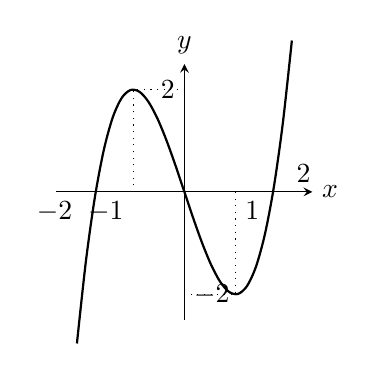
\begin{tikzpicture}[scale=0.65, >=stealth]
\draw[->] (-2.5, 0) -- (2.5, 0) node[right] {$x$};
\draw[->] (0, -2.5) -- (0, 2.5) node[above] {$y$};
\draw[domain=-2.1:2.1, smooth, variable=\x, thick] plot ({\x}, {\x*\x*\x - 3*\x});
\draw[dotted] (-1, 0) -- (-1, 2) -- (0, 2);
\draw[dotted] (1, 0) -- (1, -2) -- (0, -2);
\node[below left] at (-1, 0) {$-1$};
\node[below right] at (1, 0) {$1$};
\node[left] at (0, 2) {$2$};
\node[right] at (0, -2) {$-2$};
\node[below left] at (-2, 0) {$-2$};
\node[above right] at (2, 0) {$2$};
\end{tikzpicture}
\end{center}

\noindent
(1) $|p| > 2$ の時. 図から解はただ 1 つあり, これを $\alpha$ として $f(p) = \alpha^2$ となる. $\alpha^2$ は $|p|$ の単調増加関数であるから, $|p| \to 2$ をかんがえて,
\[
f(p) > 4 \quad \dots \text{①}
\]
以下, 対称性から $0 \le p \le 2$ でかんがえる. $p = 2$ の時, $x = 2, -1$ が解で,
\[
f(p) = -2 \quad \dots \text{②}
\]
となり, $0 < p < 2$ の時, 解は 3 つあり, これを $\alpha, \beta, \gamma$ ($\alpha < \beta < \gamma$) とおく.
\[
\begin{cases}
\alpha + \beta + \gamma = 0 \\
\alpha \beta \gamma = p \\
\beta(\alpha + \gamma) + \alpha \gamma = -3
\end{cases}
\implies
\begin{cases}
-t s = p \\
s - t^2 = -3
\end{cases}
\quad (s = \alpha \gamma, t = \alpha + \gamma) \quad \dots *
\]
から, $f(p) = s = t^2 - 3$ となる. $p = 0$ の時 $t = 0$ となるから, この時 $\min f(p) = -3$ となる. \hfill $\dots$ ③

\noindent
①, ②, ③ から, $\min f(p) = -3$ \quad (又 $f(p) = t^2 - 3$ は $p=2$ でも成立)

\bigskip

\noindent
(2) $y = g(x)$ が奇関数だから, $y = f(p)$ は偶関数である. よって $0 \le p$ でかんがえる.

\medskip
\noindent
$1^\circ \ 0 \le p \le 2$ の時

\noindent
$t$ から, $t = -\beta$ で, $\beta$ は $p$ の単調減少関数だから, $t$ は $p$ の単調増加関数であり, $t = h(p)$ とおくと,
\[
\begin{cases}
h(0) = 0, \quad h(2) = 1 \\
h'(p) > 0
\end{cases}
\]
となり, $0 \le h(p) \le 1$ である.
\[
f'(p) = 2t \frac{dt}{dp} = 2 h(p) \cdot h'(p) > 0 \quad \dots \text{④}
\]
又, $*$ から $s$ を消して
\[
p = -t(t^2 - 3)
\]
だから両辺 $p$ で微分して
\[
1 = -3t^2 \cdot t' + 3t' \quad \therefore \frac{1}{3} = (1 - t^2) \cdot t'
\]
もう1回 $p$ で微分して
\[
0 = t''(1 - t^2) - 2t \cdot (t')^2
\]
$0 \le t \le 1$ から, $0 < p < 2$ では $t' > 0$ となるから, ④より
\[
f''(p) = 2 \{ (t')^2 + t \cdot t'' \} > 0 \quad \dots \text{⑤}
\]
となる. よって ④, ⑤ から, $0 \le p < 2$ では下に凸な単調増加関数である.

\medskip
\noindent
$2^\circ \ 2 < p$ の時

\noindent
唯一の解 $\alpha$ として, $f(p) = \alpha^2$, $p = \alpha^3 - 3\alpha$ だから, $1^\circ$ と同じく $p$ で微分して
\[
1 = (3\alpha^2 - 3)\alpha' \quad \dots \text{⑥}
\]
\[
0 = (\alpha^2 - 1)\alpha'' + 2\alpha(\alpha')^2
\]
となり, $2 < \alpha$ から $\alpha' > 0$ で,
\begin{align*}
f'(p) &= 2\alpha \cdot \alpha' > 0 \\
f''(p) &= 2(\alpha' \cdot \alpha' + \alpha \cdot \alpha'') \\
&= 2 \left\{ (\alpha')^2 + \alpha \frac{-2\alpha(\alpha')^2}{\alpha^2 - 1} \right\} \quad (\because \text{⑥}) \\
&= 2(\alpha')^2 \frac{-(\alpha^2 + 1)}{\alpha^2 - 1} < 0
\end{align*}
となるから, $p > 2$ の時は上に凸な単調増加関数. 又, $f(p) \to +\infty \ (p \to +\infty)$ である.

\noindent
以上からグラフは下図.

\begin{center}
\begin{tikzpicture}[scale=0.8, >=stealth]
\draw[->] (-3.5, 0) -- (3.5, 0) node[right] {$p$};
\draw[->] (0, -3.5) -- (0, 4.5) node[above] {$y$};

\fill (0, -3) circle (2pt) node[below right] {$-3$};

\draw[thick, domain=0:2, smooth] plot (\x, {0.25*\x*\x - 3});
\draw[thick, domain=-2:0, smooth] plot (\x, {0.25*\x*\x - 3});

\draw[dotted] (2, 0) -- (2, -2) -- (0, -2);
\draw[dotted] (-2, 0) -- (-2, -2) -- (0, -2);
\fill (2, -2) circle (2pt);
\fill (-2, -2) circle (2pt);

\node[above] at (2, 0) {$2$};
\node[above] at (-2, 0) {$-2$};
\node[right] at (0, -2) {$-2$};

\draw[thick, domain=2:3.2, smooth] plot (\x, {-2 + 3*sqrt(\x - 2)});
\draw[thick, domain=-3.2:-2, smooth] plot (\x, {-2 + 3*sqrt(-\x - 2)});

\draw[dotted] (-3.5, 4) -- (3.5, 4);
\node[left] at (0, 4) {$4$};
\draw[dotted] (2, 0) -- (2, 4);
\draw[dotted] (-2, 0) -- (-2, 4);
\draw[fill=white] (2, 4) circle (2pt);
\draw[fill=white] (-2, 4) circle (2pt);

\node[below right] at (0,0) {$0$};
\end{tikzpicture}
\end{center}

\end{document}
